\documentclass{article}
\usepackage[utf8]{inputenc}
\usepackage{color}
\newcommand{\lighttodo}[1]{\textcolor{red}{#1}}
\newcommand{\todo}[1]{\lighttodo{\textbf{[TODO: #1]}}}
\usepackage{amsmath}
\usepackage{amssymb}
\usepackage{ifthen}
\usepackage{tikz}
\usetikzlibrary{arrows,shapes}

\definecolor{lightgray}{rgb}{0.8,0.8,0.8}
\definecolor{lightgrey}{rgb}{0.8,0.8,0.8}

\tikzstyle{boxed ph}=[]
\tikzstyle{sort}=[fill=lightgray,rounded corners]
\tikzstyle{process}=[circle,draw,minimum size=15pt,fill=white,
font=\footnotesize,inner sep=1pt]
\tikzstyle{black process}=[process, fill=black,text=white, font=\bfseries]
\tikzstyle{gray process}=[process, draw=black, fill=lightgray]
\tikzstyle{current process}=[process, draw=black, fill=lightgray]
\tikzstyle{process box}=[white,draw=black,rounded corners]
\tikzstyle{tick label}=[font=\footnotesize]
\tikzstyle{tick}=[black,-]%,densely dotted]
\tikzstyle{hit}=[->,>=angle 45]
\tikzstyle{selfhit}=[min distance=30pt,curve to]
\tikzstyle{bounce}=[densely dotted,->,>=latex]
\tikzstyle{hl}=[font=\bfseries,very thick]
\tikzstyle{hl2}=[hl]
\tikzstyle{nohl}=[font=\normalfont,thin]

\newcommand{\currentScope}{}
\newcommand{\currentSort}{}
\newcommand{\currentSortLabel}{}
\newcommand{\currentAlign}{}
\newcommand{\currentSize}{}

\newcounter{la}
\newcommand{\TSetSortLabel}[2]{
  \expandafter\repcommand\expandafter{\csname TUserSort@#1\endcsname}{#2}
}
\newcommand{\TSort}[4]{
  \renewcommand{\currentScope}{#1}
  \renewcommand{\currentSort}{#2}
  \renewcommand{\currentSize}{#3}
  \renewcommand{\currentAlign}{#4}
  \ifcsname TUserSort@\currentSort\endcsname
    \renewcommand{\currentSortLabel}{\csname TUserSort@\currentSort\endcsname}
  \else
    \renewcommand{\currentSortLabel}{\currentSort}
  \fi
  \begin{scope}[shift={\currentScope}]
  \ifthenelse{\equal{\currentAlign}{l}}{
    \filldraw[process box] (-0.5,-0.5) rectangle (0.5,\currentSize-0.5);
    \node[sort] at (-0.2,\currentSize-0.4) {\currentSortLabel};
   }{\ifthenelse{\equal{\currentAlign}{r}}{
     \filldraw[process box] (-0.5,-0.5) rectangle (0.5,\currentSize-0.5);
     \node[sort] at (0.2,\currentSize-0.4) {\currentSortLabel};
   }{
    \filldraw[process box] (-0.5,-0.5) rectangle (\currentSize-0.5,0.5);
    \ifthenelse{\equal{\currentAlign}{t}}{
      \node[sort,anchor=east] at (-0.3,0.2) {\currentSortLabel};
    }{
      \node[sort] at (-0.6,-0.2) {\currentSortLabel};
    }
   }}
  \setcounter{la}{\currentSize}
  \addtocounter{la}{-1}
  \foreach \i in {0,...,\value{la}} {
    \TProc{\i}
  }
  \end{scope}
}

\newcommand{\TTickProc}[2]{ % pos, label
  \ifthenelse{\equal{\currentAlign}{l}}{
    \draw[tick] (-0.6,#1) -- (-0.4,#1);
    \node[tick label, anchor=east] at (-0.55,#1) {#2};
   }{\ifthenelse{\equal{\currentAlign}{r}}{
    \draw[tick] (0.6,#1) -- (0.4,#1);
    \node[tick label, anchor=west] at (0.55,#1) {#2};
   }{
    \ifthenelse{\equal{\currentAlign}{t}}{
      \draw[tick] (#1,0.6) -- (#1,0.4);
      \node[tick label, anchor=south] at (#1,0.55) {#2};
    }{
      \draw[tick] (#1,-0.6) -- (#1,-0.4);
      \node[tick label, anchor=north] at (#1,-0.55) {#2};
    }
   }}
}
\newcommand{\TSetTick}[3]{
  \expandafter\repcommand\expandafter{\csname TUserTick@#1_#2\endcsname}{#3}
}

\newcommand{\myProc}[3]{
  \ifcsname TUserTick@\currentSort_#1\endcsname
    \TTickProc{#1}{\csname TUserTick@\currentSort_#1\endcsname}
  \else
    \TTickProc{#1}{#1}
  \fi
  \ifthenelse{\equal{\currentAlign}{l}\or\equal{\currentAlign}{r}}{
    \node[#2] (\currentSort_#1) at (0,#1) {#3};
  }{
    \node[#2] (\currentSort_#1) at (#1,0) {#3};
  }
}
\newcommand{\TSetProcStyle}[2]{
  \expandafter\repcommand\expandafter{\csname TUserProcStyle@#1\endcsname}{#2}
}
\newcommand{\TProc}[1]{
  \ifcsname TUserProcStyle@\currentSort_#1\endcsname
    \myProc{#1}{\csname TUserProcStyle@\currentSort_#1\endcsname}{}
  \else
    \myProc{#1}{process}{}
  \fi
}

\newcommand{\repcommand}[2]{
  \providecommand{#1}{#2}
  \renewcommand{#1}{#2}
}
\newcommand{\THit}[5]{
  \path[hit] (#1) edge[#2] (#3#4);
  \expandafter\repcommand\expandafter{\csname TBounce@#3@#5\endcsname}{#4}
}
\newcommand{\TBounce}[4]{
  (#1\csname TBounce@#1@#3\endcsname) edge[#2] (#3#4)
}

\newcommand{\TState}[1]{
  \foreach \proc in {#1} {
    \node[current process] (\proc) at (\proc.center) {};
  }
}


\usepackage{graphicx}
\usepackage{caption}
\usepackage{subcaption}

\usepackage{tikz}
\usetikzlibrary{fit}
\usetikzlibrary{arrows}
\usetikzlibrary{positioning}
\usepackage{stmaryrd}
\begin{document}

\section{Introduction}
Using mathematical modeling to address large scale problems in the world of biological regulatory networks has become increasingly necessary given the sheer quantity of data made available by improved technology. In the most general sense, modeling approaches can be thought of as being either quantitative or qualitative. Quantitative methods such as ordinary differential equations or the chemical master equation are widespread in the literature; when the model is well developed, the detail therein can be incredibly informative. However, these methods are not well suited for all applications. Quantitative models require an in depth knowledge of the reaction kinetics, demonstrate linear behaviors and generally fail as the problem size grows. The alternative approach, qualitative models, do not possess the same amount of detail but capture the essential dynamics of the system. In addition, qualitative models have a variety of analysis tools which can be applied regardless of the problem size. Gene regulation, as a sub genre of biological regulatory networks, is characterized by large numbers of interconnected species whose influences depend on passing some threshold, thus, largely sigmoidal behaviors. The application of qualitative methods to these systems can be highly advantageous to the modeler.\\

In this work, we begin by considering the qualitative framework of Process Hitting, defined briefly in Section \ref{process_hitting}. A highly flexible model, Process Hitting captures the most important dynamics of the system with a relatively simple syntax. The very structure of this syntax lends it to powerful static analysis tools which can be used to answer some of the most important questions about the model such as steady states or reachability without constructing the state space. Realistic models in gene regulation are immense and highly interconnected: even when considering a boolean space, the very enumeration of the possible states of the resulting system create a combinatorial explosion. This is a frequent obstacle in the field of computer science and has been dubbed the ``curse of dimensionality''. However, there are some questions for which one must access the underlying probability distribution associated with the Markov transitions of the qualitative model. In addition, gaining access to the probability distribution allows for a qualitative and intuitive analysis of the system as a whole. The most pervasive methods have historically been simulation-based, although there are some instances in which this becomes computationally infeasible. Here, we propose a method to solve the system by treating the Markov equations of a Process Hitting model with numerical techniques. A reduced-basis method, Proper Generalized Decomposition (PGD) can be used to overcome the curse of dimensionality and provide fast, computationally inexpensive solutions to an otherwise intractable problem, as discussed in Section \ref{PGD}. In addition, PGD has certain qualities particularly favorable for applications to gene regulatory networks. Unknown parameters can easily be incorporated into the model at the cost of another dimension, as demonstrated in Section \ref{parameter}.


\section{Methodologies}
\subsection{The Qualitative Model: Process Hitting}\label{process_hitting}
\begin{figure}

\begin{subfigure}[t]{0.3\textwidth}
   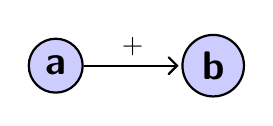
\begin{tikzpicture}[->,>=stealth',shorten >=1pt,auto,node distance=2cm,
  thick,main node/.style={circle,fill=blue!20,draw,font=\sffamily\Large\bfseries}]
  \node[main node] (a) {a};
  \node[main node] (b) [right of=a] {b};
  \path[->,>=angle 90]
(a) edge node[above]{$+$} (b);
\end{tikzpicture}
\end{subfigure}
\begin{subfigure}[b]{0.3\textwidth}
\resizebox{.9\textwidth}{!}{
 \begin{tikzpicture}[y=10cm]
  \draw (-6,0) rectangle (6,1);
  \draw [red] (0,0) -- (0,1);
    \foreach \x in {-6,-5,...,6}{
      \draw[y=1cm,thick,blue] (\x,0) -- (\x,-0.2);
      ;
    }
    \foreach \y in {0.5,1}{
      \draw[thick,blue] (0,\y) -- (-0.2,\y);
      \node at (-0.45,\y) {\y};
    }
    \coordinate (a) at (6,1);
    \coordinate (b) at (-6,0);
    \draw (b) edge[ultra thick,out=360,in=180,looseness = 2] (a);    
  \end{tikzpicture}}
  \end{subfigure}
\begin{subfigure}[b]{0.3\textwidth}
\begin{tikzpicture}
\TSort{(0,0)}{a}{2}{l}
\TSort{(2,0)}{b}{2}{r}
\THit{a_1}{very thick}{b_0}{}{b_1}
\path[bounce, bend left=25]
\TBounce{b_0}{}{b_1}{.south};
\THit{a_0}{}{b_1}{}{b_0}
\path[bounce, bend right=25]
\TBounce{b_1}{}{b_0}{.north};
\end{tikzpicture}
\end{subfigure}

\caption{Creating a Process Hitting action. In gene regulation, we consider two kinds of interactions between species: activation and inhibition. If $a$ is an activator of $b$, it is common to represent this by a signed, directed graph (left). These interactions have a characteristic form: unlike kinetic reactions, activation and inhibition usually depend on the regulator passing some threshold concentration in order to become effective (middle). Process Hitting (right) represents these reactions via actions: $a_1$ hits $b_0$ to bounce to $b_1$, indicated by a bold arrow.  Generalized dynamics attempts to create the most permissive dynamics possible for the directed graph. Therefore, the absence of $a$ effectively acts as an inhibitor, adding the action $a_0$ hits $b_1$ to bounce to $b_0$, indicated by the light arrow. In order to fully express this behavior, we associate each action with a given rate law.}
\label{PH_fig}

\end{figure}

Process hitting is a powerful yet simple tool for the analysis of large regulatory networks. Historically related to the discrete models of Ren\'{e} Thomas\cite{thomas1991regulatory} and Stuart Kauffman\cite{kauffman1969metabolic}, Process hitting attempts to address problems of scalability in classical modeling methods while maintaining the highest degree of expressiveness possible. Formally a subclass of asynchronous automata, it relies on large degrees of abstraction to describe the system as a whole. All interacting species\textemdash whether they be  enzymes, genes or proteins \textemdash are abstracted as \textit{sorts}. These sorts are then subdivided into \textit{processes}, which could represent concentration levels, spatial configuration, or any other form which has a distinct qualitative impact on the system. Processes interact with one another via \textit{actions}, in which processes \textit{hit} one another to create a \textit{bounce} to some new level of the same sort at a given rate. For gene regulatory networks, processes are often abstractions of relevant concentration ranges, discretized domains of real numbers, and actions represent activation and inhibition reactions. Figure \ref{PH_fig} illustrates how to define sorts, processes and actions from a biological understanding of an interaction. Process Hitting relies on the initial construction of the most permissive dynamics, otherwise called \textit{generalized dynamics}, which are successively enriched by the addition of \textit{cooperative sorts} in order to best capture some known biological behaviors. Cooperative sorts represent the combined effects of multiple regulators on a single target and thus must be updated such that the current state of the cooperative sort is compatible with the current state of each of its components. A visual explanation of the construction and refinement of generalized dynamics in Process hitting can be found in Figure\ref{PH_coop}.\\


\begin{figure}[h]
\centering
\begin{tikzpicture}
\TSort{(0,1)}{a}{2}{l}
\TSort{(0,-3)}{b}{2}{l}
\TSort{(6,1)}{c}{2}{r}
\TSetTick{ab}{0}{10}
\TSetTick{ab}{1}{11}
\TSetTick{ab}{2}{00}
\TSetTick{ab}{3}{01}
\TSetSortLabel{ab}{$a\wedge \neg b$}
\TSort{(2,-1)}{ab}{4}{t}

\THit{ab_0}{}{c_0}{.west}{c_1}
\THit{ab_3}{}{c_1}{.west}{c_0}
\THit{ab_1}{}{c_1}{.west}{c_0}
\THit{ab_2}{}{c_1}{.west}{c_0}

\THit{a_1}{bend left}{ab_2}{.north}{ab_0}
\THit{a_1}{bend left}{ab_3}{.north}{ab_1}
\THit{a_0}{bend left}{ab_0}{.north}{ab_2}
\THit{a_0}{bend left}{ab_1}{.north}{ab_3}
\path[bounce, bend right=20]
\TBounce{ab_2}{}{ab_0}{.north east}
\TBounce{ab_3}{}{ab_1}{.north east}
;
\path[bounce, bend left=80, distance=30]
\TBounce{ab_0}{}{ab_2}{.west}
\TBounce{ab_1}{}{ab_3}{.west}
;

\THit{b_0}{bend right}{ab_1}{.south}{ab_0}
\THit{b_0}{bend right}{ab_3}{.south}{ab_2}
\THit{b_1}{bend right}{ab_0}{.south}{ab_1}
\THit{b_1}{bend right}{ab_2}{.south}{ab_3}
\path[bounce,bend left]
\TBounce{ab_1}{}{ab_0}{.east}
\TBounce{ab_3}{}{ab_2}{.east}
;
\path[bounce,bend right]
\TBounce{ab_0}{}{ab_1}{.west}
\TBounce{ab_2}{}{ab_3}{.west}
;

\path[bounce, bend left]
\TBounce{c_0}{}{c_1}{.south}

;
\path[bounce, bend right]
\TBounce{c_1}{}{c_0}{.north}
;
\TState{a_1,b_0,ab_1,c_0}
\end{tikzpicture}
\caption{Refinement of a model via Cooperative Sorts. Generalized dynamics are unable to express logical gates in which multiple species exhibit combined effects on a target, such as $a\wedge \neg b$. In order to add these combined interactions, we must refine the Process Hitting model with cooperative sorts. Here, we have created the cooperative sort $ab$ which is updated by $a$ and $b$ such that it reflects the current state of the system.}
\label{PH_coop}
\end{figure}

Although this is a very simplistic representation of the inner kinetics of a biological process, Process Hitting semantics allow us to easily model interactions with only partial knowledge of the logical functions encoded therein and pave the way for powerful static analysis techniques in order to study fixed points, reachability and cut sets which determine minimum criteria for reachability, in spite of the present combinatorial explosion \cite{FPMR13-CS2Bio, PMR10-TCSB}. Furthermore, these tools are freely available in a software called PINT. We will not attempt to expound upon the details of Process hitting here but, rather, point those interested towards \cite{PMR10-TCSB} for a formal and thorough description. As we progress to a biological application in Section \ref{bio_application}, greater clarity will be given to the concepts described above.


\subsection{Treating Qualitative Systems with Numerical Techniques}

In order to address Process Hitting's global results, that is, the full and complete description of the systems behavior given an initial condition, we must consider the framework in a stochastic context. Process hitting actions move the system from one state, $z$, to another at a given propensity which depends on only the current state and time, or $a(z,t)$. As a memoryless random walk, each action corresponds to a Markov equation which tracks the net change in the probability of existing at a certain state and time: 
\[
\frac{\partial \Phi(z,t)}{\partial t} = \sum_j  a_j(z\prime,t)\Phi(z\prime,t) -\sum_k a_k(z,t)\Phi(z,t)
\]
The result is a system of linear, time dependent, partial differential equations, defined given an initial condition and boundary conditions. The solution is a multivariate Bernoulli distribution in which exactly one of the K outcomes is successful, or 1-in-K. This differs substantially from the multivariate Gaussian distribution in that all of the indecies are permutable, a particularly challenging characteristic of the Process Hitting structure in terms of numerical solvers. Some of the most famous and broadly used techniques for addressing problems such as these have been simulation based. While this does avoid constructing the full state space, simulation can become computationally expensive with respect to run-time and available memory. An alternative approach is the direct application of a numerical method to the Markov equations. Here, we propose Proper Generalized Decomposition (PGD) as an effective and well suited technique for gene regulatory networks.
\subsection{Proper Generalized Decomposition}\label{PGD}
Proper Generalized Decomposition \cite{chinesta2011overview,chinesta2013pgd} is a reduced basis technique which assumes that the target, in this case, the probability distribution, can be written as a sum of a product of separable functions.
\[
 \Phi(z,t)\cong \sum_{j=1}^{M}F_1^j(z_1)\cdots F_2^j(z_2)\cdots F_{N_{sp}}^j(z_{N_{sp}}) \cdot F_t(t)
\]
PGD is performed iteratively, starting at some arbitrary guess and searching for sets of functions, one vector at a time, which will minimize the residual of the running sum. These functions are colloquially called ``modes'', however, since the only objective is the reduction of the residual, there is no underlying notion that they represent the greatest source of variance, as is the case with Principal Component Analysis. Although the accuracy increases with every addition, we assume that only a limited number, $M$, of sets of functions are needed to capture the behavior of the system. If we consider a network of $N_{sp}$ sorts with $N$ processes, the resulting dimensionality is the $M$ sum of $N_{sp}$ functions of size $N$, or $M(N\times N_{sp})$ in contrast to the original $N_{sp}^N$. We have not changed the actual size of the state space but, rather, re-ordered it such that only one $N\times1$ vector, usually on the scale of 2 or 3, must be addressed at any given time. \todo{Should I include image here? reorganization of cubes?} Since all operations can be performed by canonical techniques and are highly parallelizable, iterations are generally fast and computationally inexpensive.

\section{Application to a Biological Network}\label{bio_application}

It is easier to understand the concepts of Process hitting and PGD, as well as to see their individual and combined benefits, when seen ``in action'' in the context of a realistic application towards a gene regulatory network. Here, we investigate a medium scale model of the ErbB signaling pathway which regulates a cells transition from G1 to S life phase, an important checkpoint which determines whether a cell should divide, delay division or enter a quiescent state. Over expression of ErbB is associated with many kinds of cancer, and drugs which target it and its receptor are common treatments for breast, lung and colon cancers. The directed graph for this network was taken from \cite{Sahin09}, where twenty species interact according to Boolean rules. We begin our application by constructing a Process Hitting model from this Boolean predecessor, taking the most permissive, generalized dynamics, followed by its refinement via the incorporation of cooperative sorts. The impact that this refinement has on both the static analysis and application of PGD will be investigated, both in terms of expressiveness and complexity. Finally, the potential of PGD's capacity to easily incorporate unknown variables will be demonstrated by taking into account that a particular reaction's rate law is disputed within the literature.\\

\begin{table}[h!]
\centering
  \begin{tabular}{|c|c|c|c|}
  \hline
    \textbf{Model} & \textbf{Fixed points} & $EGF_0$ & $EGF_1$ \\
  \hline
    Gen. Dynam. & 0 & True & True \\
  \hline
    Refined & 3 & False & True \\
  \hline

  \end{tabular}
   \caption{Results for ErbB models using generalized dynamics and a refinement with cooperative sorts. In order to be considered a functioning model, no signal should be able to propagate when the system is universally inactive, including the input EGF, indicated by $EGF_0$. However, in the presence of EGF, $EGF_1$, pRB should be able to activate. We see that, while the generalized dynamics were able to propagate a signal from EGF to pRB, it was not able to prevent sporadic activation of pRB, nor find any fixed points.}
   \label{egf}

\end{table}
The translation of a Boolean model to the generalized dynamics of Process Hitting is relatively straight forward, as shown in Figure \ref{PH_fig}: the absence of an activator effectively serves as an inhibitor and vice versa. The formal relationship between Boolean networks and Process Hitting can be found in \cite{FPIMR12-CMSB}. Refinement captures the suggested logical gate rules from \cite{Sahin09} via cooperative sorts. The structure of the system clearly indicates two species of experimental interest: EGF as an input, having no predecessor, and pRB as output, having no successor. Therefore, we can easily formulate simple reachability criteria in order to perform sanity checks on our model. We consider a system ``at rest'', in which all components begin in their inactive state. If no changes are made on the input protein, EGF, we expect no change to occur in the output. However if EFG is introduced, the signal should propagate to the output, pRB. Results from static analysis, shown in Table \ref{egf} provide good evidence that the generalized dynamics are too permissive and do not accurately capture the biological behaviors which are essential for a functioning model: not only are we are unable to find any fixed points within the system, but the protein pRB may become sporadicly activated in a globally inactive system. By including cooperative sorts, we recapture these vital phenomena, finding three fixed points and passing both sanity checks.


\subsection{Cooperative Sorts in the context of PGD}
The Markov Equations of the Process Hitting actions provide a system of PDEs to which we can apply PGD. Each species occupies a dimension of the state space. With two processes to each sort, the final problem is of size $2^{20}$, or over one million possible states. The underlying probability distribution is a function of these species and time. Our goal is to approximate this solution by a summation of separable functions 
\[
 \Phi(z,t)\cong \sum_{j=1}^{M}F_1^j(EGF)\cdots F_N^j(pRB)
\]
 In the case of a Process Hitting containing only the generalized dynamics, this is an appropriate and accurate method. However, once cooperative sorts are incorporated into the qualitative model, the species can no longer be represented by separable functions. To satisfy the enriched model, we may simply combine those dimensions which participate in cooperative sorts. While this does create vectors which grow exponentially, it is very rare that a single cooperative sort contains more than three or four elements. As we combine the state spaces, the error associated with PGD as compared to the solution obtained from simulation techniques decreases, figure \ref{error_coop}. But what is to be done when one species participates in multiple cooperative sorts? When the dimensions of these cooperative sorts are combined, we return to the most accurate representation of the system. Again, while it is possible to experience exponential growth, this is also a very biologically implaussible situation.\\
 
\begin{figure}[h!]
\centering
 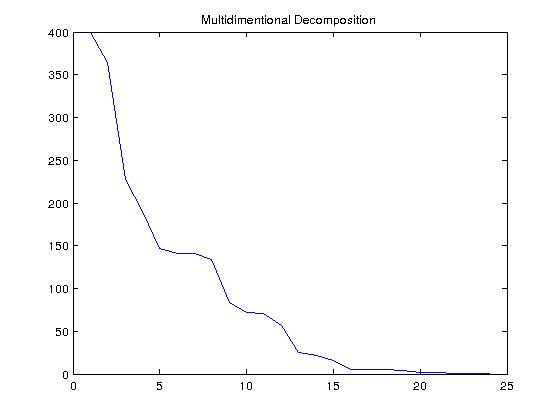
\includegraphics[width=0.5\textwidth]{singular_full.jpg}
 \caption{Error inherent in the model decreases with the increased incorporation of combined state spaces. In this case, error is judged as the Euclidian distance from the averaged results of simulation for 1000 trials.}
 \label{error_coop}
\end{figure}

The solutions that we obtain from PGD are approximations of the full solution of the problem created by Process Hitting. From these probability distributions, we are able to make fast analysis of global behaviors of the system: rather than being limited to asking the questions answerable using static analysis, a modeler can watch the system evolve through time and make general statements on the qualitative behavior. Previously undetectable elements such as limit cycles can be found, as well as temporal features.

\subsection{Incorporation of Unknown Parameters}\label{parameter}
It is often the case, especially in a growing field such as geneomics, that elements of a regulatory network are disputed or unknown. Researchers may come to very different conclusions about the parameters which fit a particular system. With simulation techniques, each new set of parameters requires a full repetition of all of the trials, limiting the modeler and leading to ad hoc choices made for the sake of feasibility. However, PGD offers a simple way of incorporating these unknown parameters directly into the model, making it possible to obtain an approximative solution for a range of values all at once\cite{chinesta2010use}. The parameter is encoded as one of the separable spaces and is included at the cost of one dimension added to the overall solution space. For our example, perhaps one of the regulating reactions is difficult to study separately from the system as a whole, say, interactions involving p27 and p21. Since these proteins are involved in both inhibiting and activating relationships, their behavior will largely influence the expression of pRB. We would like to incorporate many potential values of the action firing rate $r$ into our model, anywhere between two times faster and two times slower than the other reactions in the system. In order to do so, our decomposition of $\Phi(z,t)$ is changed slightly in order to accommodate the parameter for the range of possible values discretized into tenths:
\[
 \Phi(z,t)\cong \sum_{j=1}^{M}F_1^j(z_1)\cdots F_2^j(z_2)\cdots F_{N_{sp}}^j(z_{N_{sp}}) \cdot F_t(t)F_r(r)
\]
While simulation run time grows linearly with each element, 40 times longer since there are 40 values in the discretization, to obtain a result, we are able to derive a solution in \todo{X} by using PGD. In figure \ref{compare_par}, we see three solutions for the protein pRB given different values of the parameter $r$.

\begin{figure}[h!]
\centering
 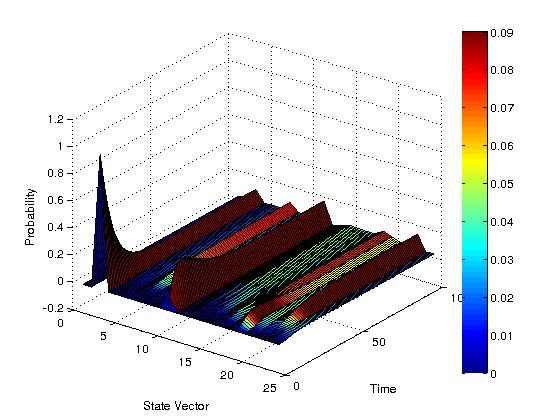
\includegraphics[width=0.25\textwidth]{pgd_normal.jpg}
  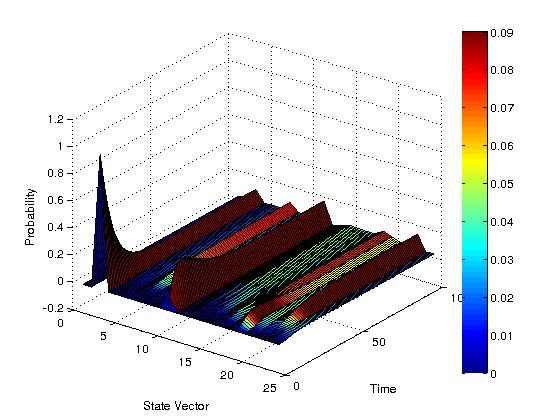
\includegraphics[width=0.25\textwidth]{pgd_normal.jpg}
 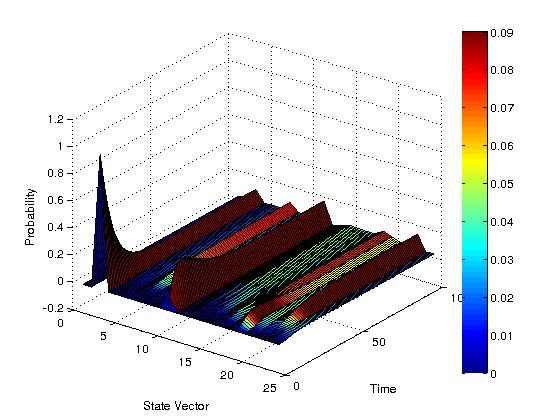
\includegraphics[width=0.25\textwidth]{pgd_normal.jpg}
 \caption{Change in the behavior of pRB given different values for the firing rates of any interaction involving the proteins p21 or p27. We imagine a scenario in which these behaviors cannot be studied separately from the system at large, and therefore must be estimated or incorporated into the model as parameters themselves. Considering that the value could be anywhere between two times slower or two times faster than the rates of the other interactions, we include functions of $r$, $F(r)$, into the decomposition of $\Phi$. Here, we see three samples of the resulting PGD solution for the output protein pRB: $1.8$ times slower (left), equal rates (center), and $1.8$ times faster (right).}
  \label{compare_par}

\end{figure} 

\section{Conclusion and Final Remarks}
In the case of gene regulatory networks, there are many reasons why a modeler might choose the application of qualitative methods, one of which is Process Hitting. Process Hitting offers many advantages for large scale, which are often the more realistic, systems in the form of static analysis tools. These analysis tools alone, however, cannot provide the complete and intuitive solution of the system as a full probability distribution for each state over time. By translating Process hitting actions to Markov equations, we are able to treat a system of PDEs directly. Proper Generalized Decomposition has proven efficient in solving Process Hitting models. As opposed to simulation techniques, which have been historically been the preferred methodology, PGD can provide full solutions, including multiple unknown paramters, with a single run. Here, we have shown some of the potential of this method, applying a combination of static analysis and numerical tools in order to maximize the expressiveness and understnading of a qualitative model. Only the basic elements of Process Hitting have been incorporated into the Markov equations considered, that is, actions with simple rate laws. Including temporal and varied stochastic features into these equations would further increase its potential.

\bibliographystyle{ouvrage-hermes}
\bibliography{biblio}

\end{document}
